\documentclass[10pt]{article}
\usepackage[T1]{fontenc}
\usepackage{lmodern,amsmath,amssymb,booktabs,array,graphicx,tikz,pgfplots}
\usepackage[paperwidth=190mm,paperheight=224mm,margin=10mm]{geometry}
\usepackage[hidelinks]{hyperref}
\hypersetup{pdfauthor={},pdftitle={Monochrome mathematical illustrations: semiconductor-health identifiability}}
\usetikzlibrary{arrows.meta,positioning,calc,patterns}
\pgfplotsset{compat=1.18}
\newcommand{\trans}{^{\mathsf T}}\newcommand{\R}{\mathbb R}
\newcommand{\one}{\mathbf 1}\newcommand{\zero}{\mathbf 0}
\DeclareMathOperator{\rank}{rank}\DeclareMathOperator{\range}{range}
\DeclareMathOperator{\diag}{diag}\DeclareMathOperator{\Cov}{Cov}
\DeclareMathOperator{\Var}{Var}\DeclareMathOperator{\spanop}{span}
\newcommand{\FigureNote}{Visualization code prepared with assistance from OpenAI Codex.}
\pagestyle{empty}\setlength{\parindent}{0pt}
\tikzset{
 every picture/.style={font=\fontsize{9}{11}\selectfont,>=Latex},
 every node/.style={font=\fontsize{9}{11}\selectfont,inner sep=2pt},
 head/.style={font=\fontsize{9.5}{12}\selectfont\bfseries,anchor=west},
 tinytext/.style={font=\fontsize{8}{10}\selectfont},eq/.style={align=center},
 wire/.style={draw=black,line width=.5pt},arr/.style={->,black,line width=.65pt},
 device/.style={draw,fill=white,minimum width=1.1cm,minimum height=.38cm}}
\pgfplotsset{mathaxis/.style={axis lines=left,axis line style={black,line width=.5pt},
 tick style={black},tick label style={font=\fontsize{8}{10}\selectfont},
 label style={font=\fontsize{8.5}{10}\selectfont},grid=major,
 major grid style={black!15,line width=.2pt},
 legend style={font=\fontsize{8}{10}\selectfont,draw=none,fill=white},
 every axis plot/.append style={black}}}
\newcommand{\PlateTitle}[2]{\small\textbf{Mathematical plate #1}\hfill Monochrome TikZ / PGFPlots\par
 \vspace{1.5mm}{\large\bfseries #2}\par\vspace{2mm}}
\newcommand{\PlateCaption}[1]{\par\vspace{1mm}{\fontsize{8.5}{10.5}\selectfont #1\par
 \vspace{1mm}\FigureNote\par}}

\begin{document}
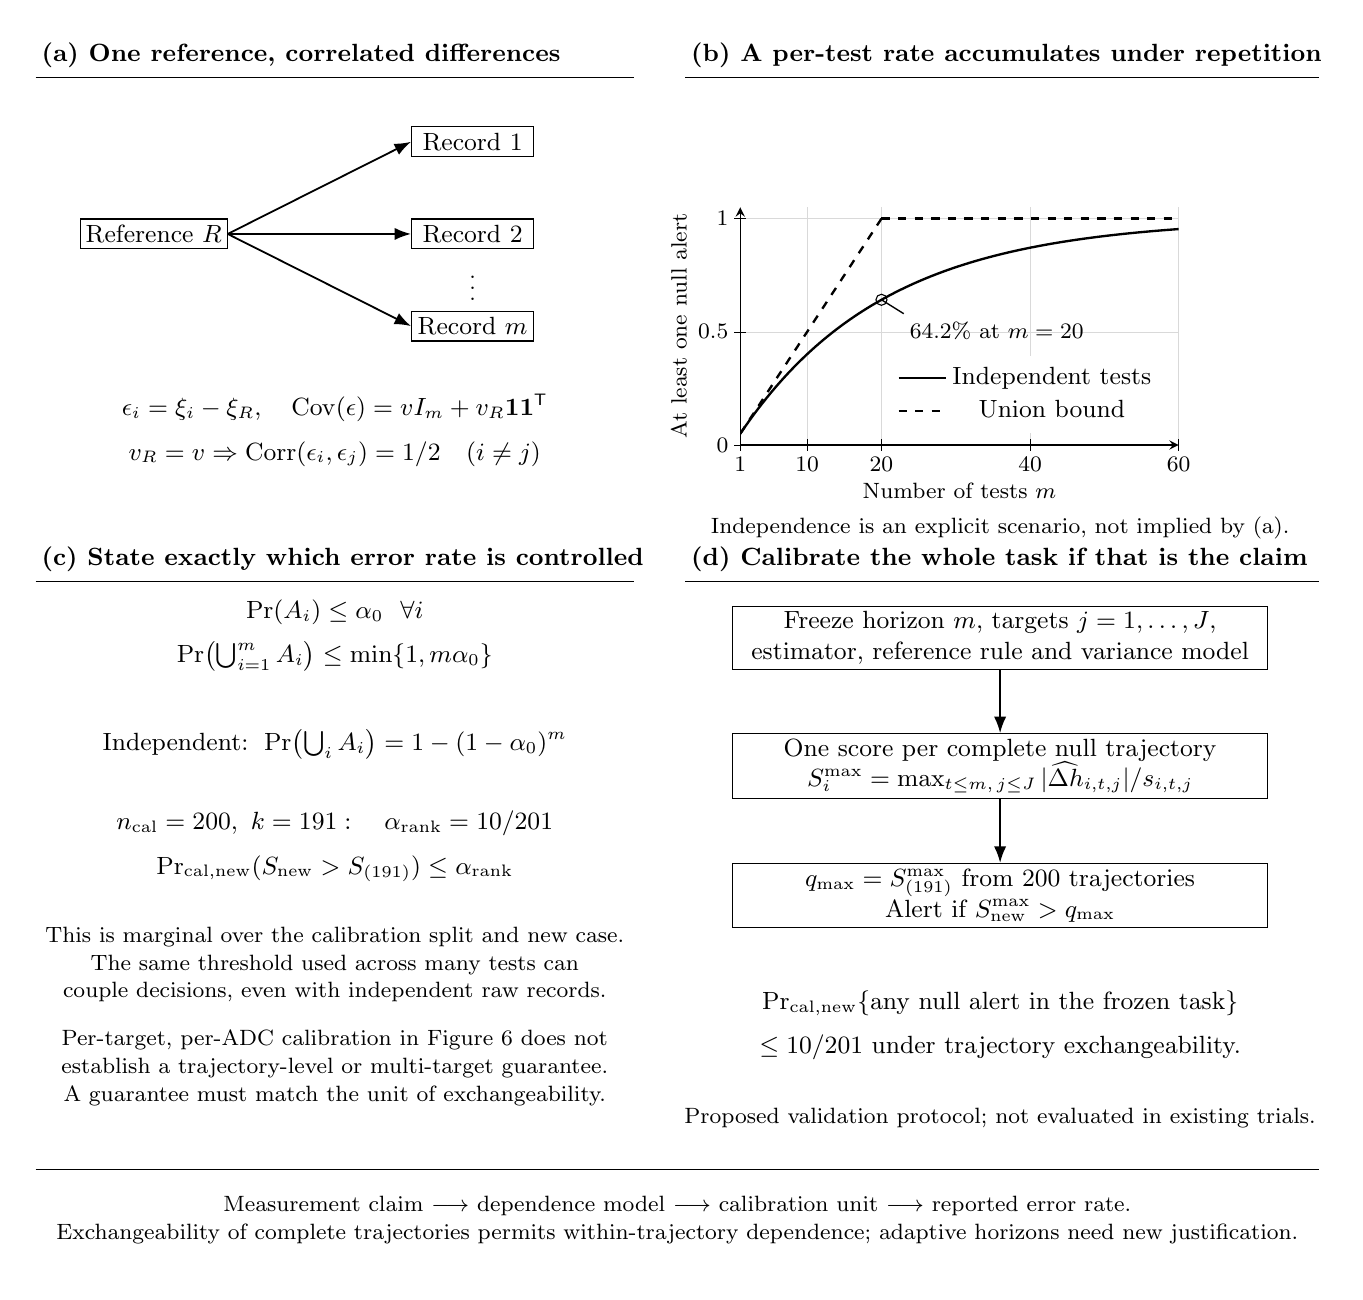
\begin{tikzpicture}[x=1cm,y=1cm]\path[use as bounding box] (0,0) rectangle (16.6,15.8);
\node[head] at (0.1,15.45){(a) One reference, correlated differences};\draw[wire] (0.1,15.17)--(7.699999999999999,15.17);
\node[head] at (8.35,15.45){(b) A per-test rate accumulates under repetition};\draw[wire] (8.35,15.17)--(16.4,15.17);
\node[device,minimum width=1.75cm] (ref) at (1.6,13.18){Reference $R$};
\node[device,minimum width=1.55cm] (m1) at (5.65,14.35){Record 1};
\node[device,minimum width=1.55cm] (m2) at (5.65,13.18){Record 2};
\node[device,minimum width=1.55cm] (mm) at (5.65,12.01){Record $m$};
\draw[arr] (ref.east)--(m1.west);\draw[arr] (ref.east)--(m2.west);\draw[arr] (ref.east)--(mm.west);
\node[tinytext] at (5.65,12.6){$\vdots$};
\node[eq] at (3.9,10.69){$\epsilon_i=\xi_i-\xi_R,\quad\Cov(\epsilon)=vI_m+v_R\one\one\trans$\\[5pt]
$v_R=v\Rightarrow\operatorname{Corr}(\epsilon_i,\epsilon_j)=1/2\quad(i\neq j)$};
\begin{axis}[mathaxis,at={(9.05cm,10.5cm)},anchor=south west,width=7.15cm,height=4.6cm,
 xmin=1,xmax=60,ymin=0,ymax=1.05,xtick={1,10,20,40,60},ytick={0,.5,1},xlabel={Number of tests $m$},ylabel={At least one null alert},
 legend style={at={(.97,.05)},anchor=south east}]
\addplot[domain=1:60,samples=100,line width=.85pt]{1-.95^x};\addlegendentry{Independent tests}
\addplot[domain=1:20,samples=40,dashed,line width=.85pt]{.05*x};
\addplot[domain=20:60,samples=2,dashed,line width=.85pt,forget plot]{1};\addlegendentry{Union bound}
\addplot[only marks,mark=o,mark size=2pt,forget plot] coordinates {(20,.641514)};
\draw[wire] (axis cs:20,.641514)--(axis cs:23,.58);
\node[tinytext,anchor=north west] at (axis cs:23,.57){$64.2\%$ at $m=20$};\end{axis}
\node[tinytext,align=center] at (12.35,9.45){Independence is an explicit scenario, not implied by (a).};
\node[head] at (0.1,9.05){(c) State exactly which error rate is controlled};\draw[wire] (0.1,8.770000000000001)--(7.699999999999999,8.770000000000001);
\node[head] at (8.35,9.05){(d) Calibrate the whole task if that is the claim};\draw[wire] (8.35,8.770000000000001)--(16.4,8.770000000000001);
\node[eq] at (3.9,8.08){$\Pr(A_i)\leq\alpha_0\ \ \forall i$\\[5pt]
$\Pr\!\left(\bigcup_{i=1}^m A_i\right)\leq\min\{1,m\alpha_0\}$};
\node[eq] at (3.9,6.7){$\text{Independent: }\Pr\!\left(\bigcup_i A_i\right)=1-(1-\alpha_0)^m$};
\node[eq] at (3.9,5.4){$n_{\mathrm{cal}}=200,\ k=191:\quad\alpha_{\mathrm{rank}}=10/201$\\[5pt]
$\Pr_{\mathrm{cal,new}}(S_{\mathrm{new}}>S_{(191)})\leq\alpha_{\mathrm{rank}}$};
\node[tinytext,align=center] at (3.9,3.9){This is marginal over the calibration split and new case.\\The same threshold used across many tests can\\couple decisions, even with independent raw records.};
\node[tinytext,align=center] at (3.9,2.59){Per-target, per-ADC calibration in Figure 6 does not\\establish a trajectory-level or multi-target guarantee.\\A guarantee must match the unit of exchangeability.};
\node[draw,align=center,minimum width=6.8cm] (traj) at (12.35,8.05){Freeze horizon $m$, targets $j=1,\ldots,J$,\\estimator, reference rule and variance model};
\node[draw,align=center,minimum width=6.8cm] (score) at (12.35,6.42){One score per complete null trajectory\\$S_i^{\max}=\max_{t\leq m,\,j\leq J}|\widehat{\Delta h}_{i,t,j}|/s_{i,t,j}$};
\node[draw,align=center,minimum width=6.8cm] (quant) at (12.35,4.78){$q_{\max}=S_{(191)}^{\max}$ from 200 trajectories\\Alert if $S_{\mathrm{new}}^{\max}>q_{\max}$};
\draw[arr] (traj.south)--(score.north);\draw[arr] (score.south)--(quant.north);
\node[eq] at (12.35,3.13){$\Pr_{\mathrm{cal,new}}\{\text{any null alert in the frozen task}\}$\\[5pt]
$\leq10/201$ under trajectory exchangeability.};
\node[tinytext,align=center] at (12.35,1.95){Proposed validation protocol; not evaluated in existing trials.};
\draw[wire] (.1,1.3)--(16.4,1.3);
\node[tinytext,align=center] at (8.25,.66){Measurement claim $\longrightarrow$ dependence model $\longrightarrow$ calibration unit $\longrightarrow$ reported error rate.\\Exchangeability of complete trajectories permits within-trajectory dependence; adaptive horizons need new justification.};
\end{tikzpicture}
\end{document}
